\chapter{音乐项目}
\label{ch:music}

\begin{introduction}
  \item 认识 P33 无源蜂鸣器：PWM 频率就是音高；
  \item 在钢琴卷帘里录入、编辑音符，理解 PPQ、速度与拍号事件；
  \item 掌握单音裁决：重叠音符按 highest/lowest/nearest 只发声一个；
  \item 会从 MIDI 文件导入旋律、把乐曲导出成 MIDI；
  \item 看懂固件如何把卷帘数据变成一段循环播放的曲子。
\end{introduction}

机器人不只会打架。音乐项目把主控板 P33 上的无源蜂鸣器变成一只喇叭：在
钢琴卷帘里录入一段旋律，PIE-Block 把它裁决成单音事件流并生成固件，板子
上电就循环演奏，SDCC 构建还会在 OLED 屏上滚动显示五线谱。这一章把卷帘
编辑、MIDI 导入导出与固件生成一次讲完。示例使用随书的
\texttt{music-twinkle.pieproj}（教材示例：小星星片段）。

\section{无源蜂鸣器：频率即音高}

主控板上的 P33 接的是一只\textbf{无源}蜂鸣器：它内部没有振荡电路，只是一
片压电陶瓷振膜（见图~\ref{fig:ch07-buzzer}），给多少频率的电信号就振出
多少频率的声音。固件用一路 PWM 驱动它——\texttt{PWM\_SET\_Frequency} 的
第一个参数是音高对应的频率，占空比固定在 5000（一半）附近：

\begin{lstlisting}[style=pieblockc,
  caption={音乐固件的发声核心：PWM 频率即音高（\texttt{music-twinkle.c} 节选）},
  label={lst:ch07-tone}]
#define MUSIC_BUZZER_CH PWMB_CH3_P33
#define MUSIC_DUTY_ON 5000
#define MUSIC_DUTY_OFF 0

static const uint16_t musicFrequencies[128] =
{
    1000, 9, 9, 10, /* ... MIDI 音高 0--127 的频率表，A4=440Hz ... */
    523, 554, 587, 622, 659, 698, 740, 784,   /* C5 起 */
    /* ... */
};

static void Music_PlayOnce(void)
{
    uint16_t i;
    MusicClock_Reset();
    for (i = 0; i < STAFF_EVENT_COUNT; i++)
    {
        MusicClock_WaitDeadline();
        if (staffPitches[i] == 0)
            Music_Stop();
        else
            PWM_SET_Frequency(MUSIC_BUZZER_CH,
                musicFrequencies[staffPitches[i]], MUSIC_DUTY_ON);
        OLEDStaff_Show(&staffSong, i);
        MusicClock_Advance(staffDurationsMs[i]);
    }
    MusicClock_WaitDeadline();
    Music_Stop();
}
\end{lstlisting}

\texttt{musicFrequencies} 表按 MIDI 音高（0--127）索引频率，$A_4=440$\,Hz
十二平均律；音高 0 表示休止，固件停掉 PWM。无源蜂鸣器的有效响应区在
数百到数千赫兹——这也是调试工程提示音的音符都落在 C6 以上的原因
（见第~\ref{ch:debugproj}~章）。

\begin{figure}[htbp]
  \centering
  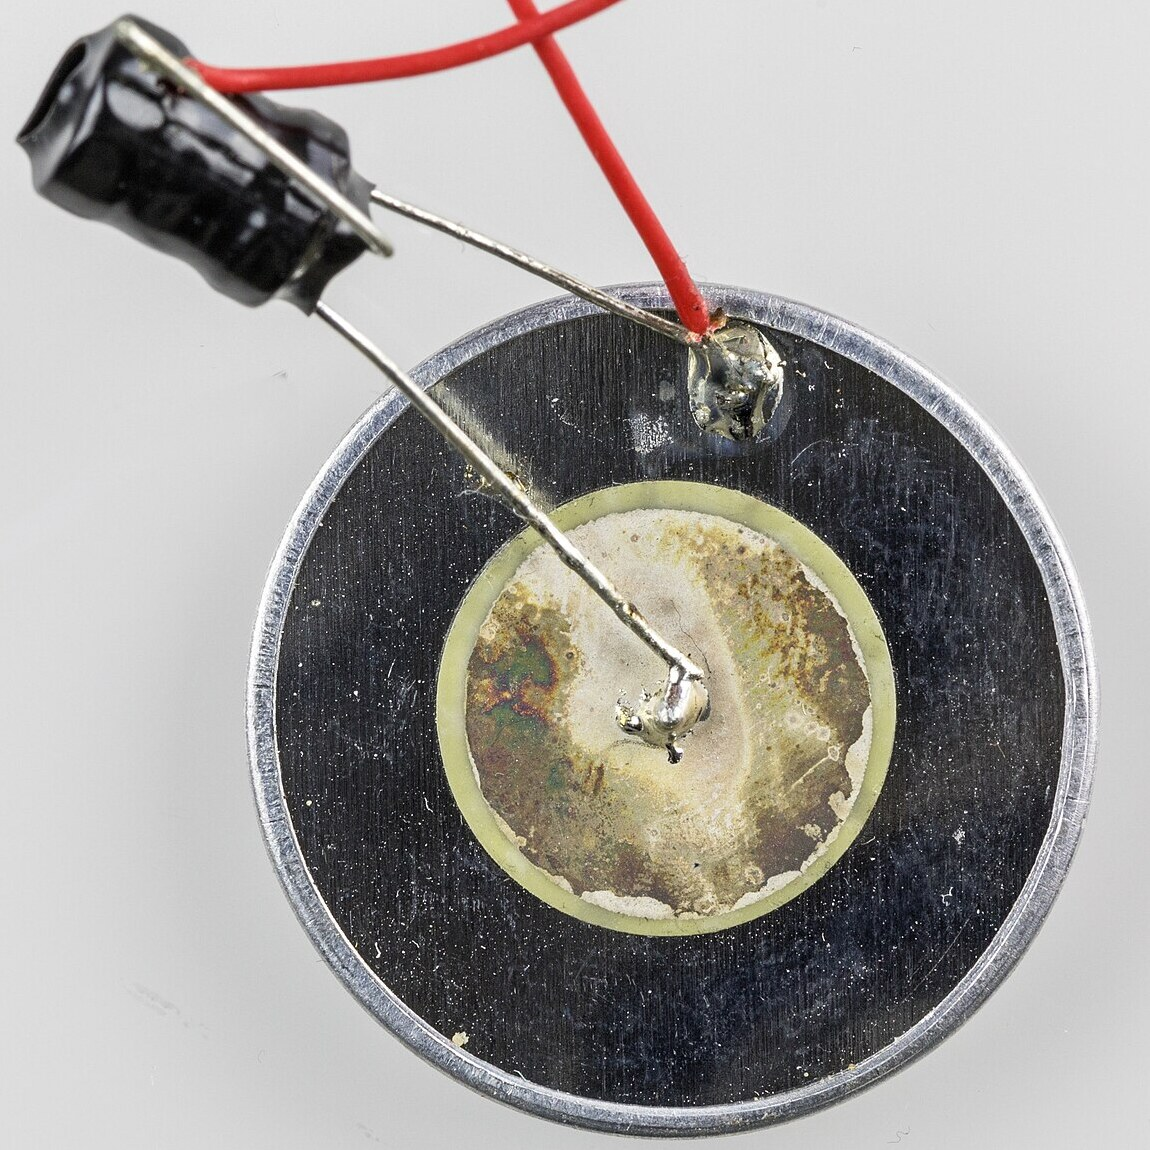
\includegraphics[width=0.62\linewidth]{image/ch07/7-2-buzzer.jpg}
  \caption{压电蜂鸣器的发声核心：黄铜基板上的压电陶瓷片。施加交变电压时
  金属片随电压频率振动而发声——固件里改 PWM 频率就是改音高。无源蜂鸣器
  自身不带振荡电路，音色由驱动信号决定（照片：Raimond Spekking，
  Wikimedia Commons，CC BY-SA 4.0）}
  \label{fig:ch07-buzzer}
\end{figure}

\section{钢琴卷帘}

音乐项目的第 1 步就是钢琴卷帘编辑器（图~\ref{fig:ch07-roll}）：横轴是
时间（以 tick 计），纵轴是音高，左边一列钢琴键对照音高，画布上的色块
就是音符。

\begin{figure}[htbp]
  \centering
  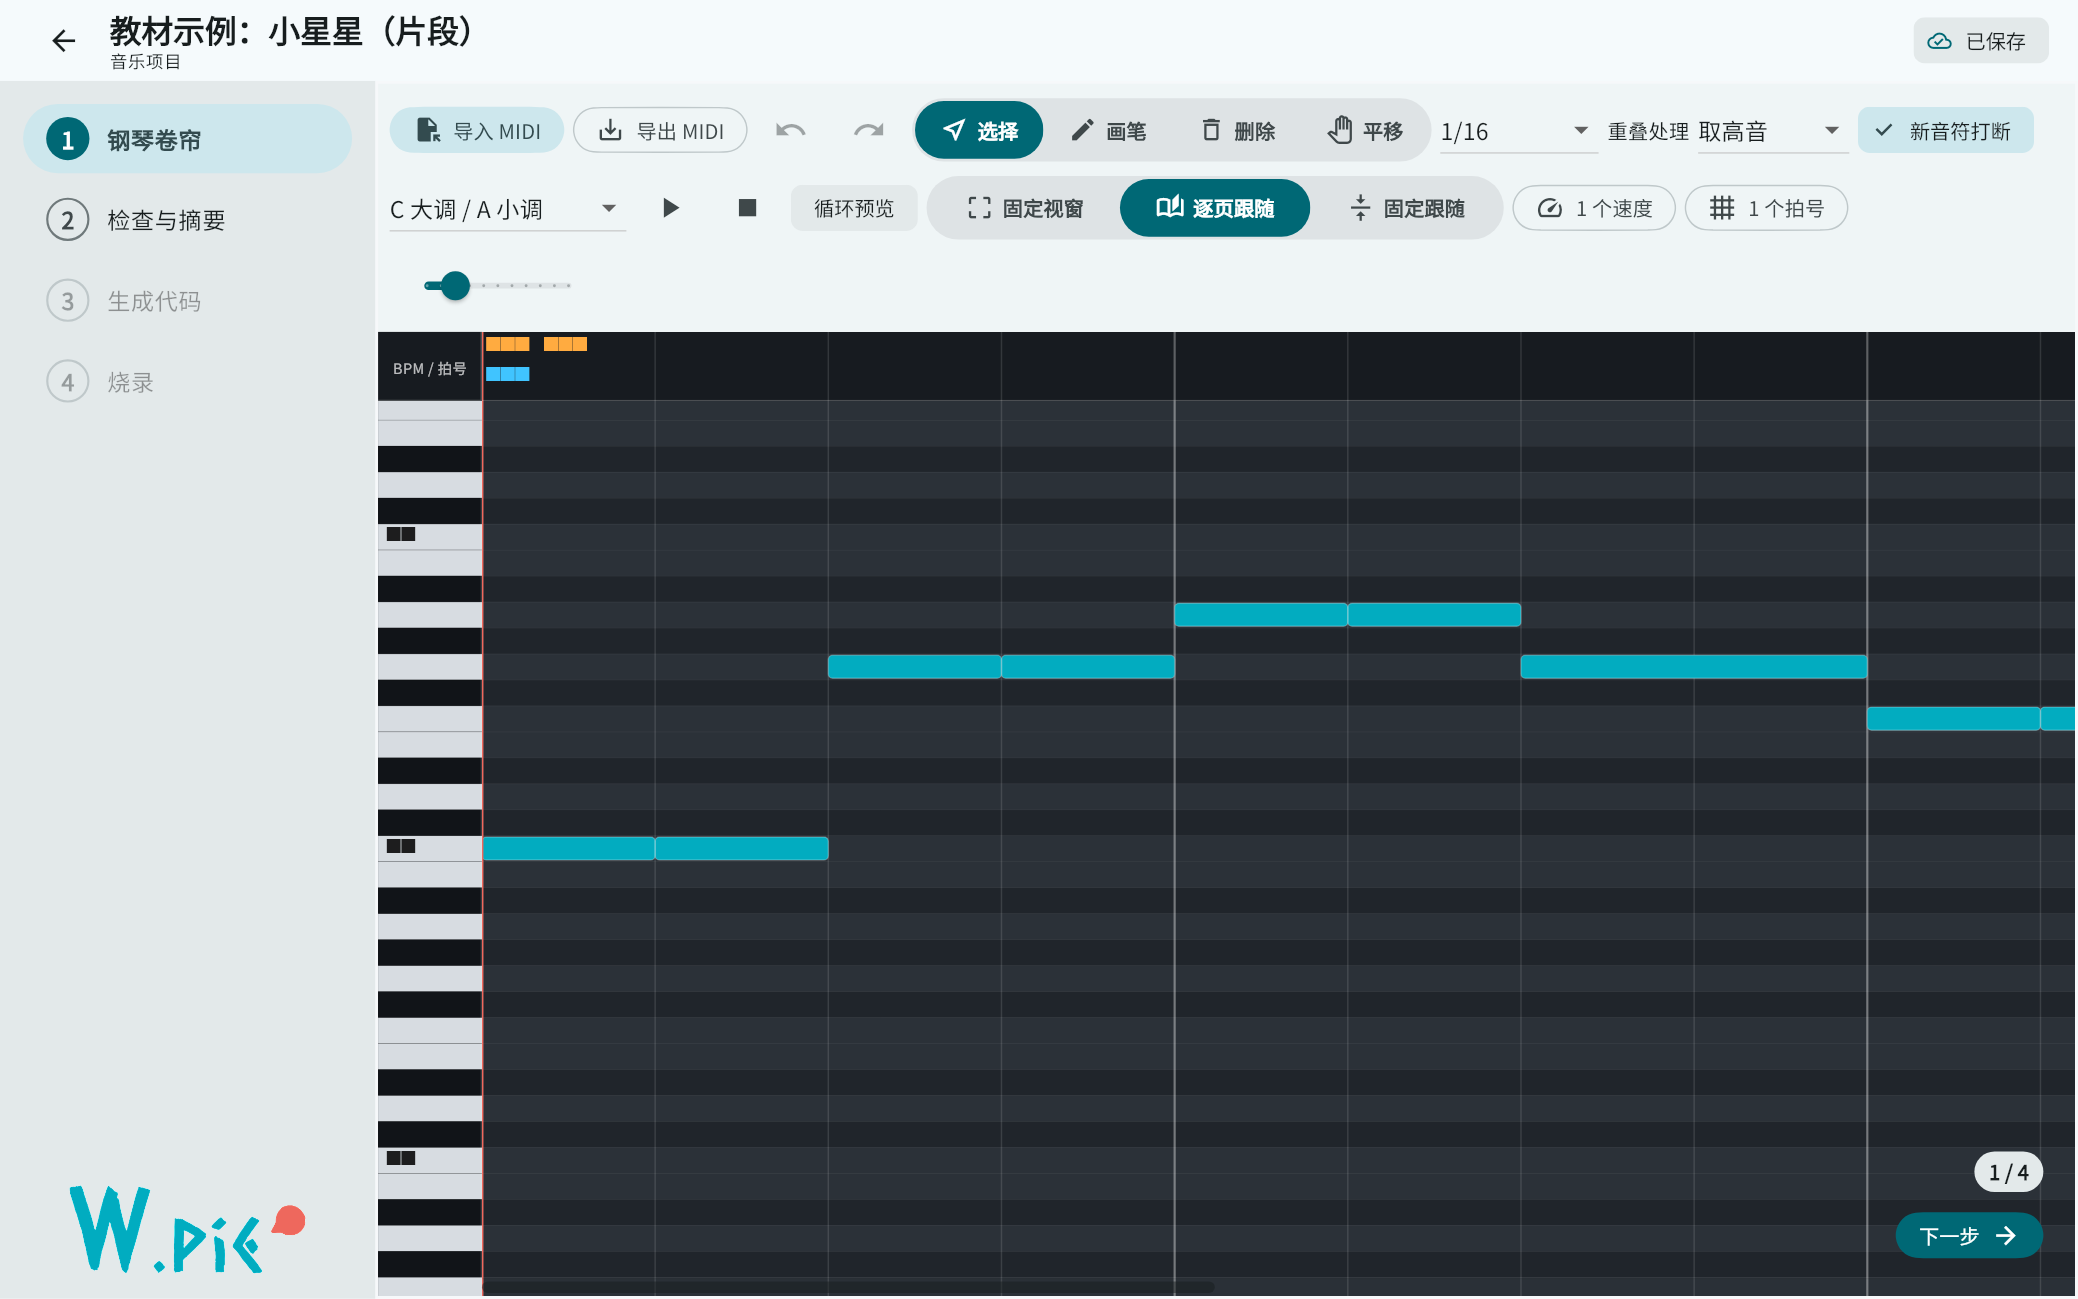
\includegraphics[width=0.98\linewidth]{image/ch07/7-1-music-editor.png}
  \caption{钢琴卷帘编辑器：工具栏上有 MIDI 导入导出、四种编辑工具、
  网格吸附与重叠处理；第二行是播放控制、视窗跟随与速度/拍号事件}
  \label{fig:ch07-roll}
\end{figure}

\subsection{工具与吸附}

编辑工具有四种：\textbf{选择}（点选、框选音符）、\textbf{画笔}（在网格
上按下即新建音符，拖动改变时值）、\textbf{删除}与\textbf{平移}（整段
移动选中的音符）。网格吸附决定新建与拖动对齐的刻度：1/16 表示十六分
音符，也可以选三连音或“不吸附”。撤销/重做（Ctrl+Z / Ctrl+Y）在编辑
过程中始终可用。

\subsection{PPQ、速度与拍号}

时间的最小单位是 tick。\textbf{PPQ}（ticks per quarter，每四分音符的
tick 数，1--32767）决定时间分辨率：480 PPQ 时一个四分音符是 480 tick，
一个八分音符是 240。曲子的快慢由\textbf{速度事件}（每四分音符的微秒数）
决定：500000 微秒即 120 BPM。\textbf{拍号事件}（分子/分母）与调号影响
五线谱显示。两类事件都必须从 tick 0 开始并严格递增，校验器会检查。

\subsection{播放与视窗}

顶部的播放控制支持从任意位置试听；“循环预览”在编辑区内循环播放选中
片段；视窗可以在“固定”“固定跟随”“逐页跟随”之间切换——播放时卷帘
自动跟随曲子的当前位置。预览由 Dart 端合成，与固件共享同一套单音裁决，
听到的就是板子会放的样子。

\section{单音裁决：重叠了让谁发声}

P33 蜂鸣器同一时刻只能发一个音，而卷帘允许音符重叠（和弦、复调、甚至
同一音高的叠写）。“重叠处理”决定裁决规则：

\begin{itemize}
  \item \textbf{highest}：取音高最高的音符发声；
  \item \textbf{lowest}：取音高最低的音符发声；
  \item \textbf{nearest}：取最接近上一个有效发声音高的音符（曲首没有
        参照时取最高音），旋律的连贯性最好。
\end{itemize}

同一 tick 起始的一组音符按同一规则只挑一个，其余整段不发声；\textbf{新
音符打断}打开时，后起始的音符会打断仍在发声的音符，被打断的尾巴不再
发声。不发声的音符与片段在卷帘里显示为灰色——数据仍完整保留，也参与
MIDI 导出，只是固件不播放它们。裁决在\textbf{生成代码时}完成：固件里
的事件表（\texttt{staffPitches} 等）已经是裁决后的单音序列，运行时只管
按表播放，不再做任何判断。

校验器会统计重叠次数并提示“检测到 $N$ 处音符重叠，将按「××」只发声
一个”；导入带和弦的 MIDI 时，导入对话框也会让你先选裁决规则。

\section{MIDI 导入导出}

“导入 MIDI”从标准 MIDI 文件里挑一条\textbf{非鼓组的旋律轨道}，把其中的
音符换算成卷帘数据（PPQ、速度与拍号事件一并导入）；文件里如果有和弦，
按所选规则只保留一个声部。导出则反向生成标准 MIDI 文件，重叠的完整数据
也会写出——卷帘里灰色的音符在 DAW（数字音频工作站）里依然可以编辑。

音乐项目不保存原始 MIDI 字节、力度、乐器与通道信息；导出的 MIDI 按单音
裁决后的发声结果计算时值。若 MIDI 里没有可用的旋律轨道，导入会明确
报错而不是导入一条空轨。

\section{固件生成与资源约束}

音乐项目的“生成代码”页给出完整固件：单音事件表、频率表与播放循环，
SDCC 构建还附带 128$\times$64 OLED 五线谱滚动显示——音符的字形点阵在
生成期全部预算好，固件只做搬运与刷新（\texttt{OLEDStaff\_Show}）。Keil
构建不带 OLED 显示，只播放声音。

校验器对曲子的规模有三道闸：

\begin{itemize}
  \item 生成的事件片段不能超过 8192 个；
  \item 曲目总时长不能超过 20 分钟；
  \item 曲目较长时提示“五线谱固件预计约占多少 KB，接近 STC32G 低 64KB
        应用区上限”——注意主控板的应用区只有低 64KB，超长的曲子要
        缩短或减少音符。
\end{itemize}

\begin{remark}
调试工程的“提示音试听”与音乐项目共用同一份频率表与发声代码：蜂鸣器
的音色取决于驱动信号，而不取决于蜂鸣器本身——同一块板子，既能“哔”出
检查单的音型，也能完整演奏《小星星》。
\end{remark}

本章的“检查与摘要、生成代码、烧录”三步与步兵项目完全一致。下一章
深入生成代码与静态检查，看看 PIE-Block 在“按下生成”之前替你查了什么。
